\documentclass{report}
\setlength{\parskip}{0pt} % esp. entre parrafos
\setlength{\parindent}{20pt} % esp. al inicio de un parrafo
\usepackage{amsmath} % mates
\usepackage{listings}
\usepackage{xcolor}
\usepackage[sort&compress,numbers]{natbib} % referencias
\usepackage{url} % que las URLs se vean lindas
\usepackage[top=10mm,left=20mm,right=20mm,bottom=25mm]{geometry} % \textbf{\textbf{}}margenes
\usepackage{hyperref} % ligas de URLs
\usepackage{graphicx} % poner figuras
\usepackage{caption}
\usepackage{subcaption}
\usepackage[spanish]{babel} % otros idiomas
\hypersetup{
    colorlinks=true,
    linkcolor=blue,
    filecolor=blue,      
    urlcolor=blue,
}
\renewcommand{\lstlistingname}{C\'odigo}
\definecolor{codegreen}{rgb}{0,0.6,0}
\definecolor{codegray}{rgb}{0.5,0.5,0.5}
\definecolor{codepurple}{rgb}{0.58,0,0.82}
\definecolor{backcolour}{rgb}{0.95,0.95,0.92}
\lstdefinestyle{mystyle}{
    backgroundcolor=\color{backcolour},   
    commentstyle=\color{codegreen},
    keywordstyle=\color{magenta},
    numberstyle=\tiny\color{codegray},
    stringstyle=\color{codepurple},
    basicstyle=\ttfamily\footnotesize,
    breakatwhitespace=false,         
    breaklines=true,                 
    keepspaces=true,                 
    numbers=left,                    
    numbersep=5pt,                  
    showspaces=false,                
    showstringspaces=false,
    showtabs=false,                  
    tabsize=2
}
\lstset{style=mystyle}

\title{Reporte 12:\\Red Neuronal}
\author{Jorge Torres}
\date{\today}

\begin{document}

\maketitle

\chapter{Entrenamiento para N\'umeros}\label{cap1}

\section{Objetivo}

Esta actividad es una demostración básica de aprendizaje a m\'aquina: se reconocer\'an d\'igitos de im\'agenes peque\~nas en blanco y negro con una red neuronal. El objetivo consiste en estudiar de manera sistem\'atica el desempeño de la red neuronal en términos de su puntaje F (F-score en ingl\'es) para los diez d\'igitos en funci\'on de las tres probabilidades asignadas a la generaci\'on de los d\'igitos $(n, g, b)$, variando a las tres en un experimento factorial adecuado.

\section{Desarrollo}

El desarrollo de la actividad est\'a basado en el \href{https://github.com/satuelisa/Simulation/blob/master/NeuralNetwork/ann.R}{c\'odigo} implementado por E. Schaeffer, con algunas modificaciones para variar las probabilidades de generaci\'on de los d\'igitos y realizar el an\'alisis estad\'istico \cite{elisa1}. La implementaci\'on completa se puede obtener del repositorio en GitHub de J. Torres \cite{jorge1}.

Las funciones \texttt{binario} y \texttt{decimal} del c\'odigo \ref{codigo1} convierten un n\'umero decimal en binario y uno binario en decimal, respectivamente.

\begin{lstlisting}[caption=Conversiones Binario y Decimal, label=codigo1, language=R]
binario <- function(d, l) {
  b <-  rep(FALSE, l)
  while (l > 0 | d > 0) {
    b[l] <- (d %% 2 == 1)
    l <- l - 1
    d <- bitwShiftR(d, 1)
  }
  return(b)
}

decimal <- function(bits, l) {
  valor <- 0
  for (pos in 1:l) {
    valor <- valor + 2^(l - pos) * bits[pos]
  }
  return(valor)
}

df = data.frame()
\end{lstlisting}

Las l\'ineas del c\'odigo \ref{codigo2} establecen las listas de probabilidades de que los bits del mapa de bits creado sean de color negro, gris o blanco, respectivamente. Este mapa de bits se utilizar\'a para entrenar y probar la red neuronal.

\begin{lstlisting}[caption={Probabilidades de Negro, Gris y Blanco}, label=codigo2, language=R]
probn = c(0.98,0.65,0.35)
probg = c(0.95,0.75,0.55)
probb = c(0.45,0.10,0.005)
\end{lstlisting}

En el c\'odigo \ref{codigo3} se inician las iteraciones entre las listas de probabilidades y se realizan 12 repeticiones para cada iteraci\'on. Se toman los valores de un archivo de texto y las probabilidades respectivas para generar un mapa de bits con una serie de d\'igitos de manera aleatoria, como se aprecia en la figura \ref{fig1}.

\begin{figure}
    \centering
    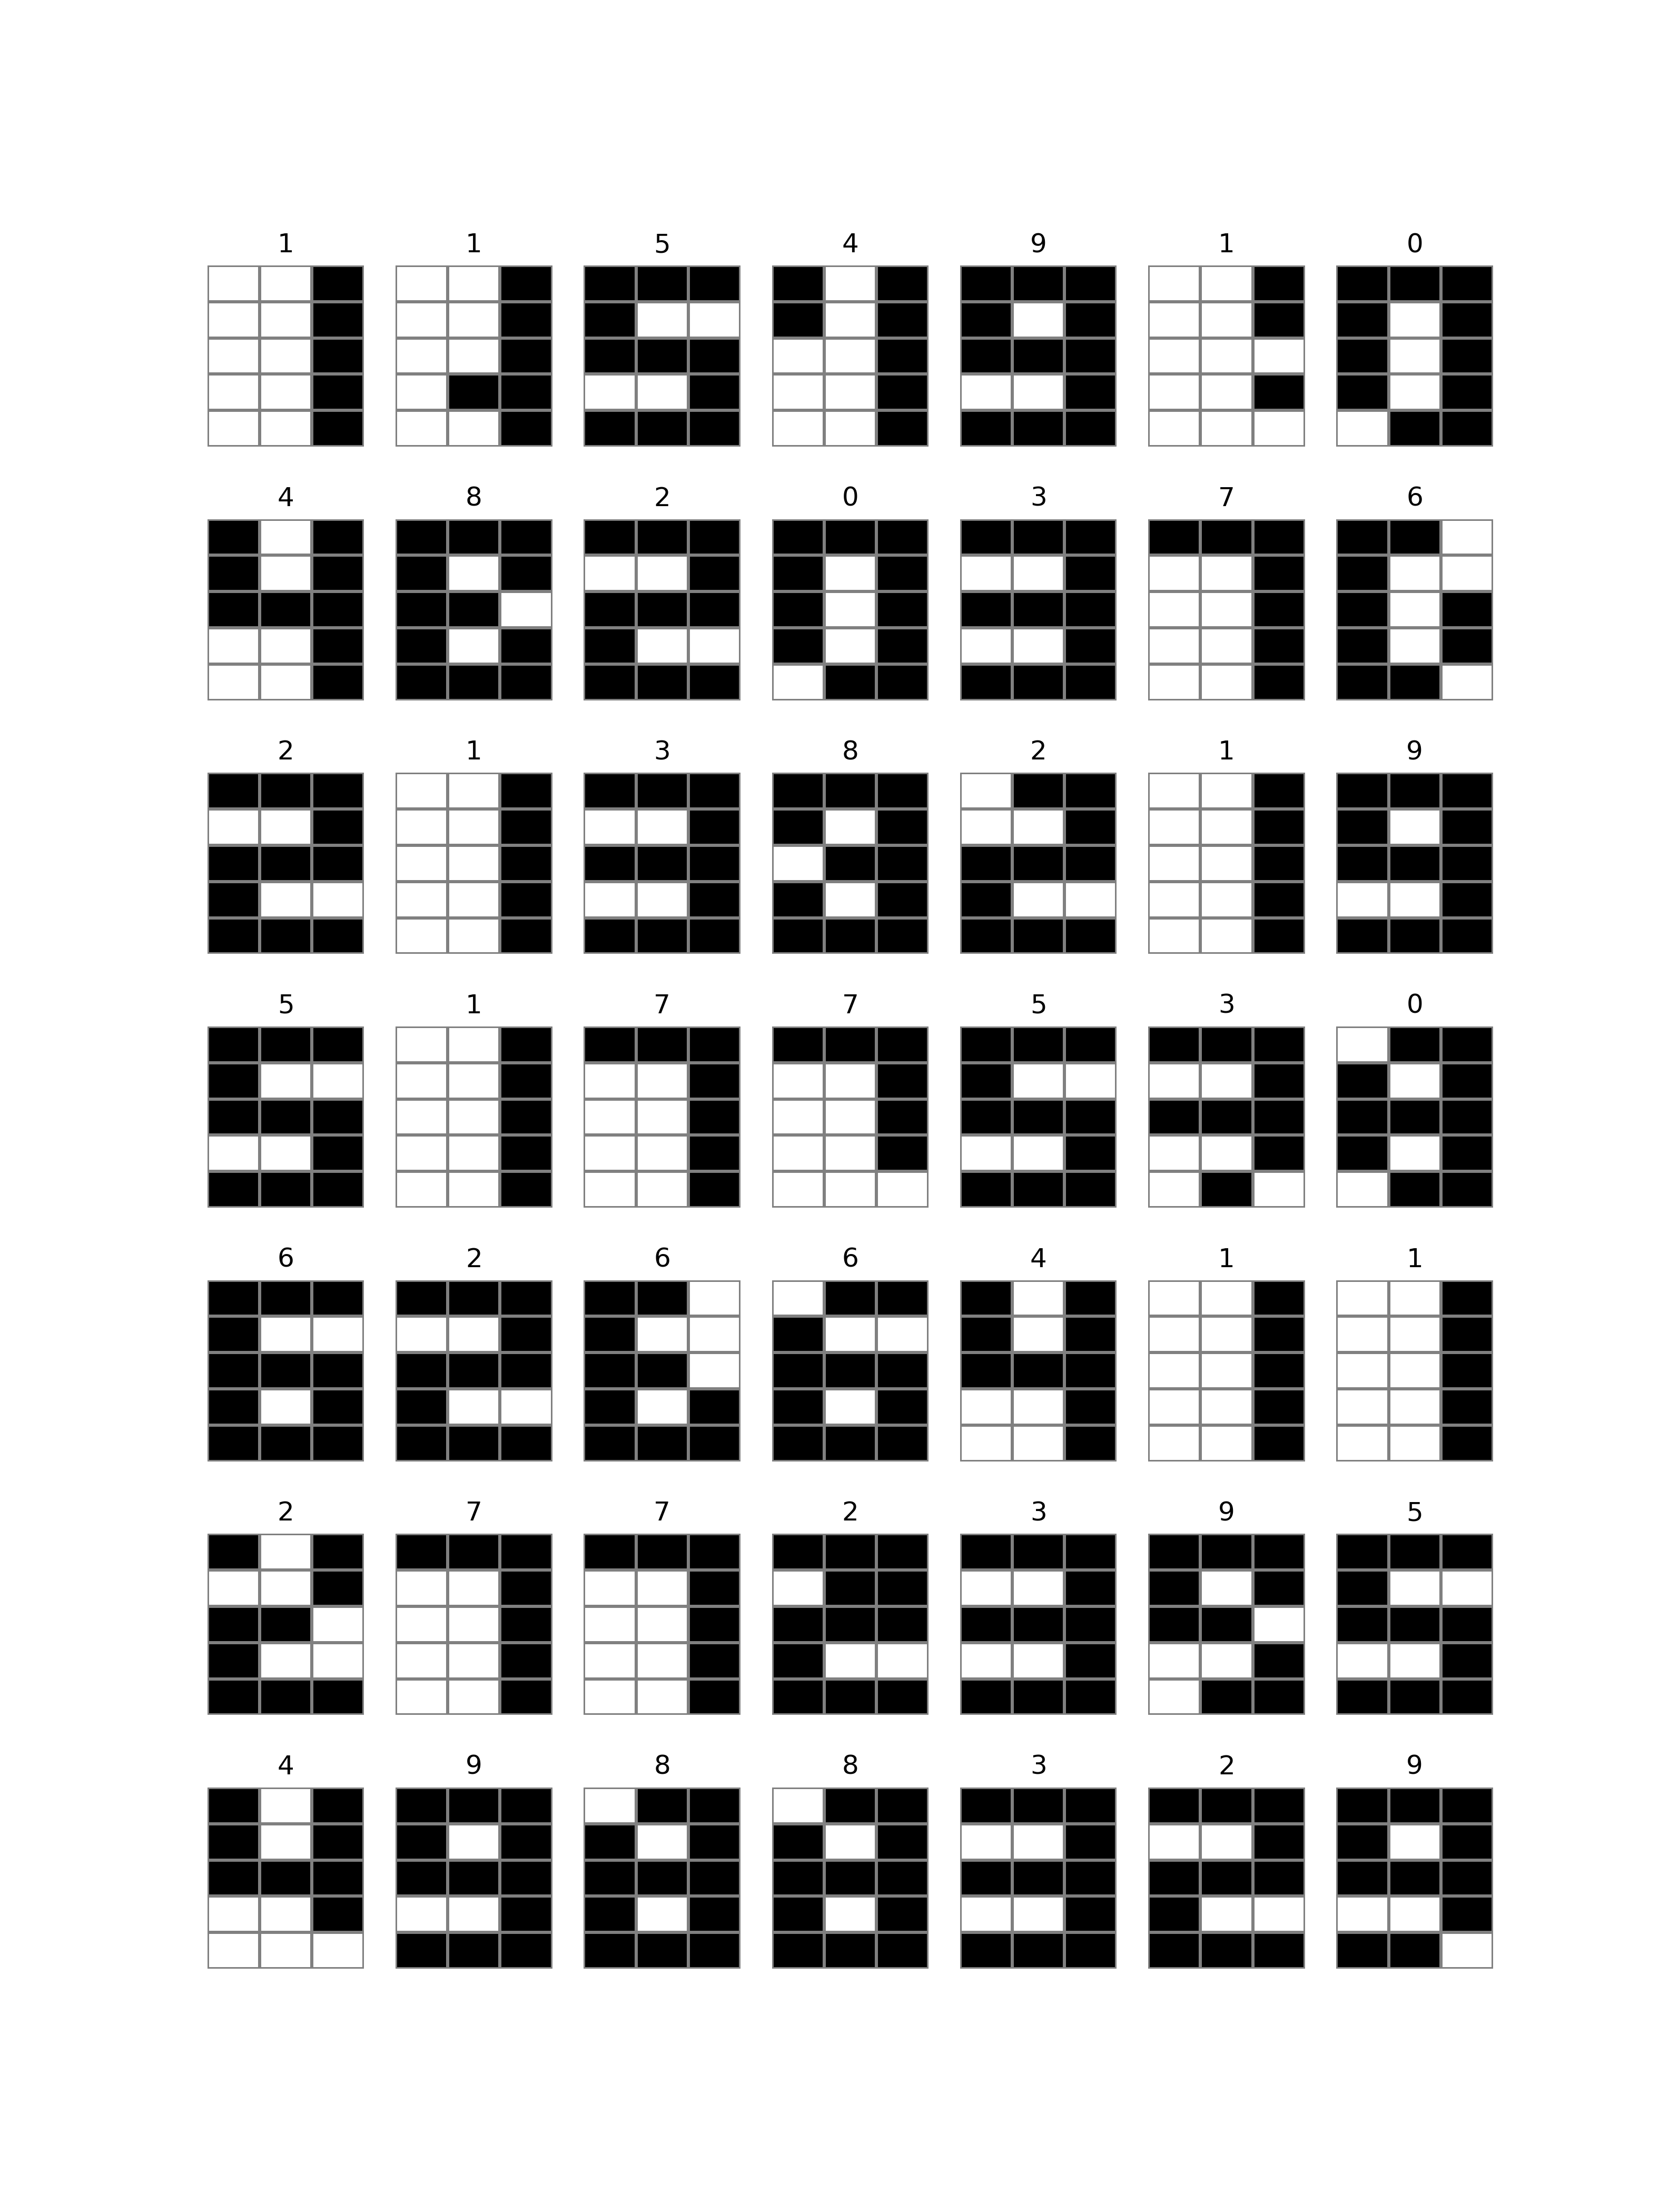
\includegraphics[width=\textwidth]{Images/p12pg.png}
    \caption{Serie de d\'igitos generados aleatoriamente, tomando las probabilidades del c\'odigo \ref{codigo2}.}
    \label{fig1}
\end{figure}

\begin{lstlisting}[caption=Generaci\'on del Mapa de Bits de los D\'igitos, label=codigo3, language=R]
for (ne in probn){
  for (g in probg){
    for (b in probb){
      for (replica in 1:12){
        modelos <- read.csv("digits.txt", sep=" ", header=FALSE, stringsAsFactors=F)
        modelos[modelos=='n'] <- ne
        modelos[modelos=='g'] <- g
        modelos[modelos=='b'] <- b
        
        r <- 5
        c <- 3
        dim <- r * c
        
        tope <- 9
        digitos <- 0:tope
        k <- length(digitos)
        contadores <- matrix(rep(0, k*(k+1)), nrow=k, ncol=(k+1))
        rownames(contadores) <- 0:tope
        colnames(contadores) <- c(0:tope, NA)
\end{lstlisting}

En el c\'odigo \ref{codigo4} se establecen la tasa de aprendizaje y el factor por el cual ir\'a disminuyendo dicha tasa en la etapa de entrenamiento. Tambi\'en se establece la cantidad de perceptrones necesarios para la red neuronal. La etapa de entrenamiento consiste en tomar d\'igitos enteros del 0 al 9 de manera aleatoria y comparar el resultado del c\'odigo \ref{codigo3} con el valor real por medio de los perceptrones. En este caso se realizan 5000 pasos de entrenamiento y se ajustan los perceptrones dependiendo de la validez del resultado.

\begin{lstlisting}[caption=Etapa de Entrenamiento de los Perceptrones, label=codigo4, language=R]
        tasa <- 0.15
        tranqui <- 0.99
        n <- floor(log(k-1, 2)) + 1
        neuronas <- matrix(runif(n * dim), nrow=n, ncol=dim)
        
        for (t in 1:5000) {
          d <- sample(0:tope, 1)
          pixeles <- runif(dim) < modelos[d + 1,]
          correcto <- binario(d, n)
          for (i in 1:n) {
            w <- neuronas[i,]
            deseada <- correcto[i]
            resultado <- sum(w * pixeles) >= 0
            if (deseada != resultado) {
              ajuste <- tasa * (deseada - resultado)
              tasa <- tranqui * tasa
              neuronas[i,] <- w + ajuste * pixeles
            }
          }
        }
\end{lstlisting}

La etapa de prueba consiste en tomar los perceptrones obtenidos de la etapa de entrenamiento y aplicarlos directamente al mapa de bits. De esta forma, la red neuronal determinar\'a a qu\'e valor pertenece cada d\'igito generado. Se hace un conteo de todos los resultados obtenidos, el cual se utiliza para su posterior an\'alisis. Esto se implementa en el c\'odigo \ref{codigo5}.

\begin{lstlisting}[caption=Etapa de Prueba y Obtenci\'on de Resultados, label=codigo5, language=R]
        for (t in 1:300) {
          d <- sample(0:tope, 1)
          pixeles <- runif(dim) < modelos[d + 1,]
          correcto <- binario(d, n)
          salida <- rep(FALSE, n)
          for (i in 1:n) {
            w <- neuronas[i,]
            deseada <- correcto[i]
            resultado <- sum(w * pixeles) >= 0
            salida[i] <- resultado
          }
          r <- min(decimal(salida, n), k)
          contadores[d+1, r+1] <- contadores[d+1, r+1] + 1
        }
\end{lstlisting}

\newpage

Para obtener el puntaje F y realizar las pruebas estad\'isticas, se utiliza la ecuaci\'on \ref{eq1}, obtenida de la lectura en pruebas estad\'isticas de Shmueli \cite{f1}, y se aplica para cada grupo de probabilidades por medio del c\'odigo \ref{codigo6}.

\begin{equation}\label{eq1}
    F=2\frac{(precision)(recall)}{precision+recall}
\end{equation}

\begin{lstlisting}[caption=Obtenci\'on del Puntaje F, label=codigo6, language=R]
        precision = diag(contadores) / colSums(contadores[,1:10])
        recall = diag(contadores) / rowSums(contadores)
        fscore = (2 * precision * recall) / (precision + recall)
        result = c(ne, g, b, replica, fscore)
        df = rbind(df, result)
      }
    }
  }
}
\end{lstlisting}

\section{Resultados}

Las distribuciones de los puntajes f (F-score) para las 12 repeticiones de cada grupo de probabilidades se muestran en la figura \ref{fig2}. Se puede observar c\'omo aumenta el puntaje para los grupos en los que la probabilidad de bits negros es mayor y la probabilidad de bits blancos es menor. Esto es de esperarse, pues en general se crear\'ian im\'agenes de los d\'igitos m\'as n\'itidas y con menos ruido.\\

Los puntajes obtenidos no parecen seguir una distribuci\'on normal, por lo que se ha realizado una prueba de tipo \texttt{Shapiro-Wilk} para comprobar dicho supuesto, mientras que se realiza una prueba de \texttt{Levene} para determinar la homogeneidad de varianza entre los grupos. Los resultados se muestran en el cuadro \ref{cuadro1}. Los ``outliers'' se refieren a la cantidad de valores at\'ipicos en los grupos. Se puede observar que, para la mayor\'ia de grupos, el valor $p$ obtenido es menor a $0.05$, por lo que no tienen una distribuci\'on normal.\\

Debido a esta distribuci\'on, se ha optado por realizar una prueba del tipo \texttt{Kruskall-Wallis} para determinar si existe una diferencia significativa en el puntaje F dependiente de las probabilidades iniciales. Los resultados se muestran en el cuadro \ref{cuadro2}. Se obtiene un valor $p$ mucho menor a $0.05$, por lo que se puede saber que la diferencia en el puntaje F es significativa al variar las probabilidades.

\begin{table}[ht]
\centering
\caption{Resultados de las pruebas de normalidad y homogeneidad de varianza.}
\smallskip

\begin{tabular}{ |p{2.1cm}|p{5cm}|}
 \hline
 Outliers & $47$ \\
 \hline
 Normalidad por grupo & $0.35/0.55/0.005$: $p$ = $1.72\times 10^{-6}$ $0.35/0.55/0.10$: $p$ = $1.81\times 10^{-4}$ $0.35/0.55/0.45$: $p$ = $1.06\times 10^{-4}$ $0.35/0.75/0.005$: $p$ = $1.62\times 10^{-7}$ $0.35/0.75/0.10$: $p$ = $2.05\times 10^{-6}$ $0.35/0.75/0.45$: $p$ = $2.43\times 10^{-4}$ $0.35/0.95/0.005$: $p$ = $2.35\times 10^{-6}$ $0.35/0.95/0.10$: $p$ = $4.48\times 10^{-6}$ $0.35/0.95/0.45$: $p$ = $2.02\times 10^{-4}$ $0.65/0.55/0.005$: $p$ = $5.30\times 10^{-5}$ $0.65/0.55/0.10$: $p$ = $2.37\times 10^{-2}$ $0.65/0.55/0.45$: $p$ = $2.31\times 10^{-2}$ $0.65/0.75/0.005$: $p$ = $3.42\times 10^{-3}$ $0.65/0.75/0.10$: $p$ = $3.93\times 10^{-4}$ $0.65/0.75/0.45$: $p$ = $1.16\times 10^{-5}$ $0.65/0.95/0.005$: $p$ = $6.09\times 10^{-3}$ $0.65/0.95/0.10$: $p$ = $8.46\times 10^{-4}$ $0.65/0.95/0.45$: $p$ = $7.73\times 10^{-5}$ $0.98/0.55/0.005$: $p$ = $6.68\times 10^{-4}$ $0.98/0.55/0.10$: $p$ = $2.58\times 10^{-1}$ $0.98/0.55/0.45$: $p$ = $4.47\times 10^{-4}$ $0.98/0.75/0.005$: $p$ = $8.90\times 10^{-6}$ $0.98/0.75/0.10$: $p$ = $1.25\times 10^{-1}$ $0.98/0.75/0.45$: $p$ = $3.07\times 10^{-3}$ $0.98/0.95/0.005$: $p$ = $8.79\times 10^{-15}$ $0.98/0.95/0.10$: $p$ = $2.38\times 10^{-6}$ $0.98/0.95/0.45$: $p$ = $1.34\times 10^{-3}$\\
 \hline
 Homogeneidad de varianza & $p$ = $3.43\times 10^{-22}$ \\
 \hline
\end{tabular}
\label{cuadro1}
\end{table}

\begin{table}[ht!]
\centering
\caption{Resultados al aplicar la prueba estadística \texttt{Kruskal Wallis}.}
\smallskip

\begin{tabular}{ |p{2.1cm}|p{2.1cm}|}
 \hline
 Chi cuadrada & Valor de $p$ \\
 \hline
 $1603.7$ & $2.2\times 10^{-16}$ \\
 \hline
\end{tabular}
\label{cuadro2}
\end{table}

\begin{figure}
    \centering
    \includegraphics[width=\textwidth]{Images/p12p_violin.png}
    \caption{Puntajes F obtenidos para todos los grupos de probabilidades.}
    \label{fig2}
\end{figure}

\newpage

\section{Conclusiones}

Como se puede observar por la gr\'afica presentada y los resultados de los an\'alisis estad\'isticos, es razonable concluir que no solamente existe una deferencia significativa en el puntaje F al variar las probabilidades iniciales, sino que esta diferencia es mucha m\'as apreciable al tener mayores probabilidades de dibujar bits negros y menores probabilidades de dibujar un bit blanco. Esto es debido a que, con tales probabilidades, e obtienen im\'agenes menos ruidosas, por lo que la red neuronal puede realizar mejores identificaciones.

\chapter{Entrenamiento para N\'umeros y S\'imbolos}

\section{Objetivo}

El objetivo del primer reto consiste en extender y entrenar la red neuronal para que reconozca, además,  por lo menos doce símbolos ASCII adicionales, aumentando la resolución de las imágenes a $5\times7$ del original de $3\times5$.

\section{Desarrollo}
El desarrollo para el primer reto es muy similar al implementado en el cap\'itulo \ref{cap1}. La diferencia est\'a en la cantidad de s\'imbolos que se utilizan y, por ende, la cantidad de perceptrones que la red neuronal necesita para las fases de entrenamiento y prueba. En el c\'odigo \ref{codigo7} se listan las probabilidades $(n, g, b)$ utilizadas, as\'i como la cantidad de d\'igitos que ahora debe reconocer la red neuronal.

\begin{lstlisting}[caption=Nuevos Par\'ametros de Operaci\'on, label=codigo7, language=R]
modelos <- read.csv("digits2.txt", sep=" ", header=FALSE, stringsAsFactors=F)
modelos[modelos=='n'] <- 0.99
modelos[modelos=='g'] <- 0.92
modelos[modelos=='b'] <- 0.002

r <- 7
c <- 5
dim <- r * c

n <- 56
w <- ceiling(sqrt(n))
h <- ceiling(n / w)

tope <- 21
digitos <- 0:tope
k <- length(digitos)
contadores <- matrix(rep(0, k*(k+1)), nrow=k, ncol=(k+1))
rownames(contadores) <- 0:tope
colnames(contadores) <- c(0:tope, NA)

n <- floor(log(k-1, 2)) + 1
neuronas <- matrix(runif(n * dim), nrow=n, ncol=dim)
\end{lstlisting}

Utilizando estos datos, el mapa de bits cuyos s\'imbolos ahora debe reconocer la red neuronal se observa en la figura \ref{fig3}.

\begin{figure}
    \centering
    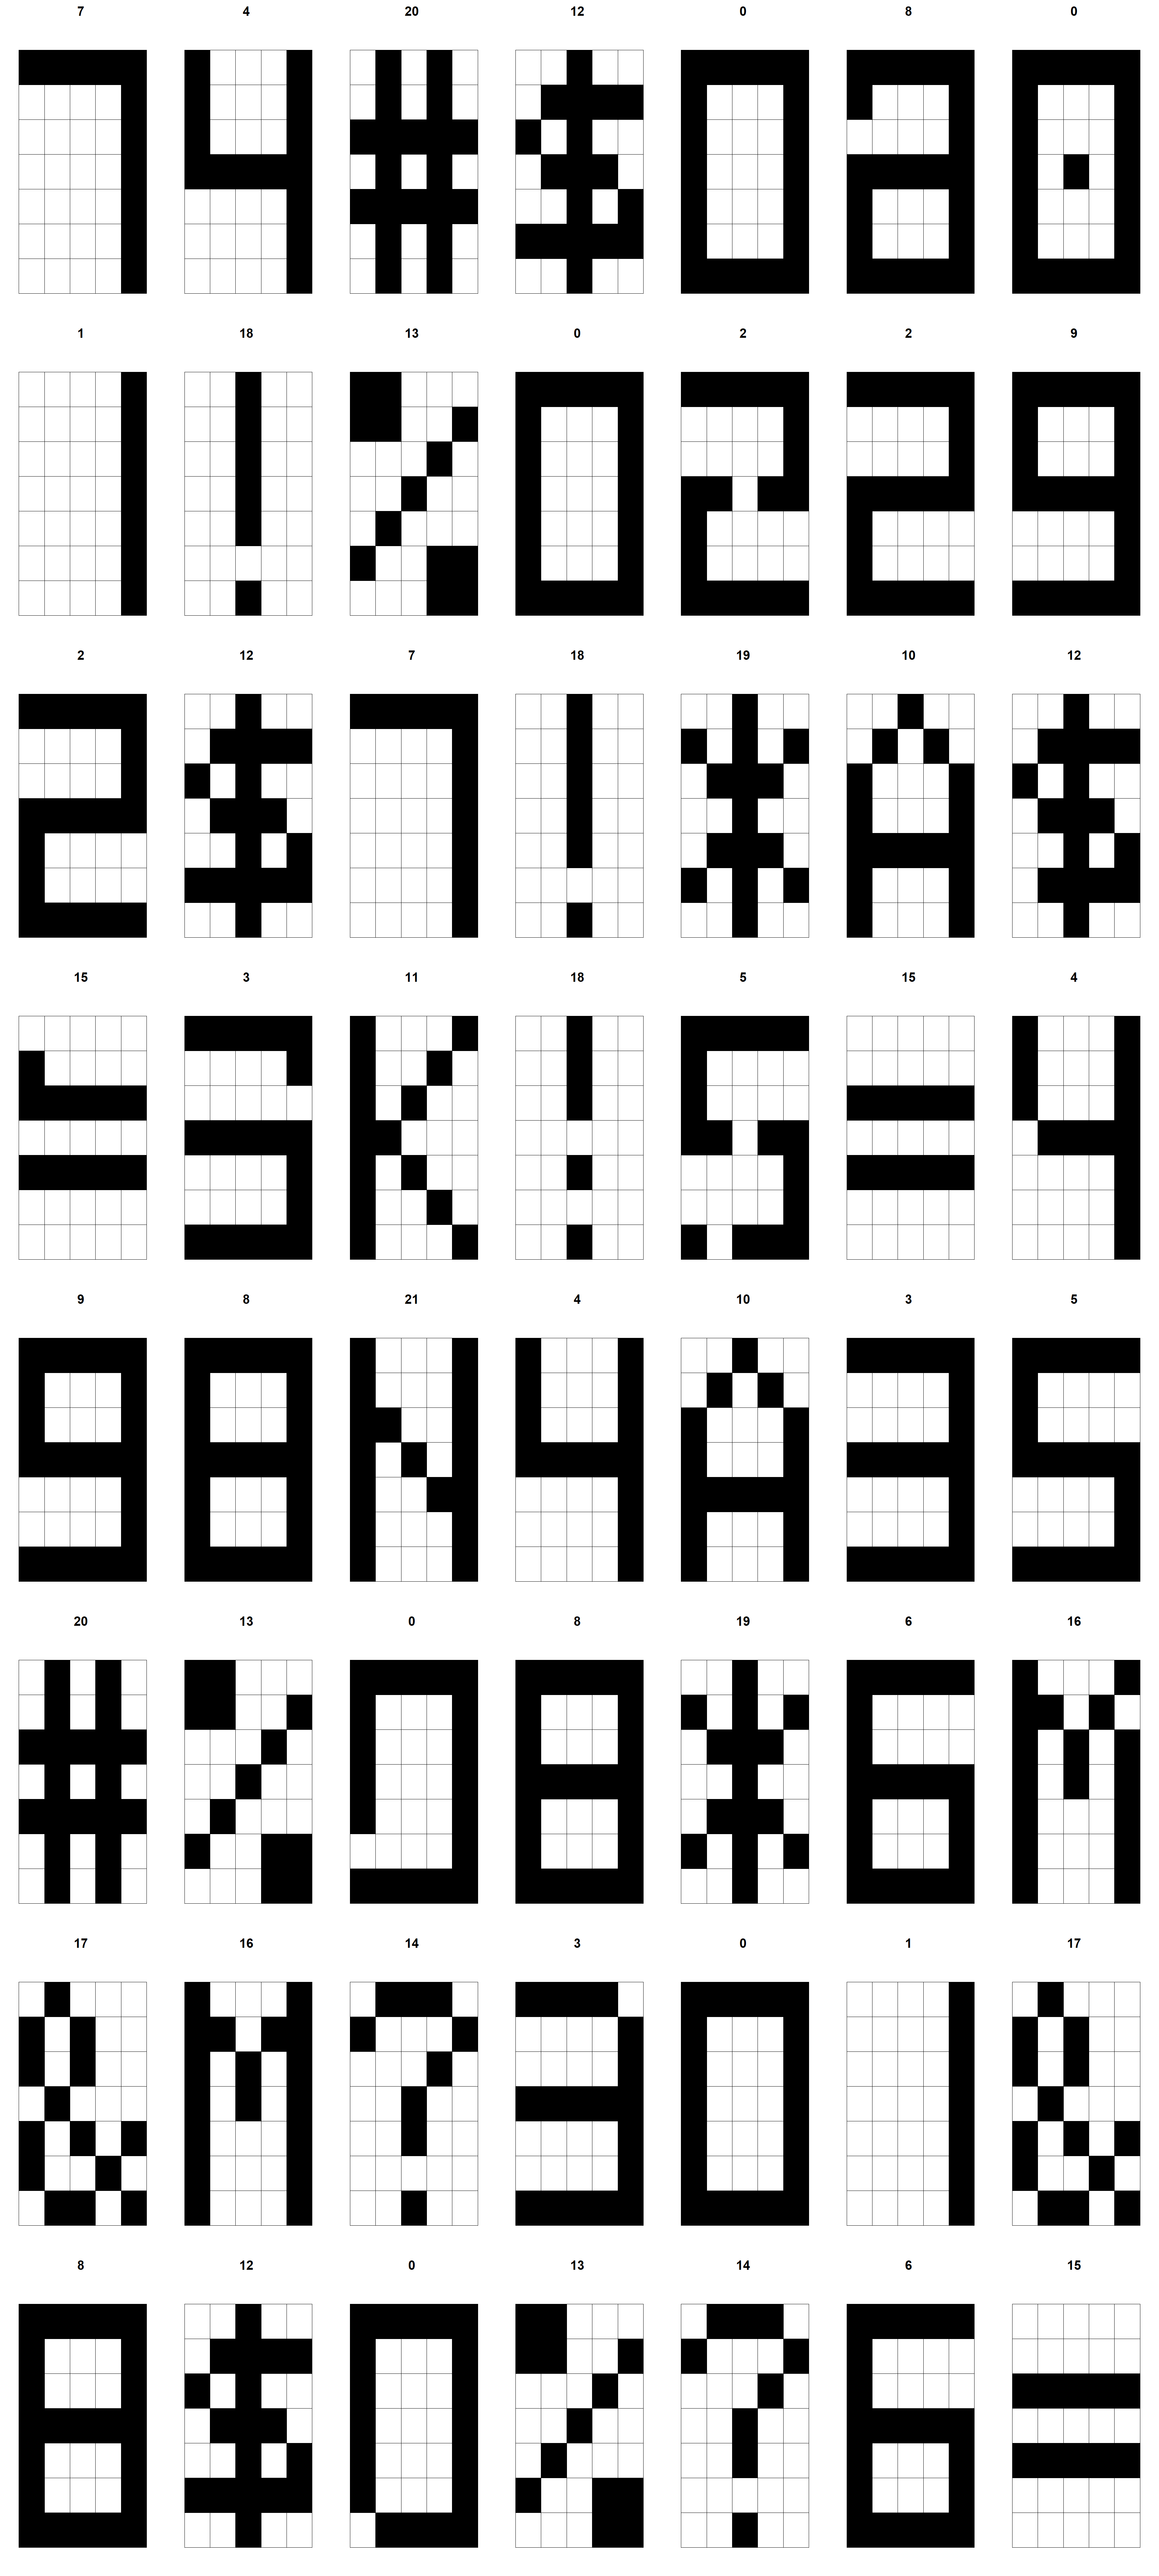
\includegraphics[width=0.6\textwidth]{Images/p12pg2.png}
    \caption{Mapa de bits a reconocer con la inclusi\'on de los nuevos s\'imbolos.}
    \label{fig3}
\end{figure}

\newpage

\section{Resultados}

Lo que se muestra en el c\'odigo \ref{codigo8} es la matriz de resultados que arroja el programa con los datos establecidos. Las filas representan el valor real de cada s\'imbolo (21 en total), mientras que las columnas representan el valor que la red neuronal interpreta. De esta forma, cada relaci\'on fila-columna representa la cantidad de veces que la red neuronal reconoce el s\'imbolo de la fila (real) como el s\'imbolo de la columna (valor interpretado). Un ejemplo bastante extremo ser\'ia la intepretaci\'on del valor 0; se puede observar c\'omo, de las 14 pruebas que hizo la red neuronal para este valor, \'unicamente 3 de ellas fueron correctas, mientras que 11 de ellas las interpreta como un valor 1.

\begin{lstlisting}[caption=Matriz de Interpretaci\'on, label=codigo8, language=R]
   0  1  2 3 4  5  6 7 8 9 10 11 12 13 14 15 16 17 18 19 20 21 <NA>
0  3 11  0 0 0  0  0 0 0 0  0  0  0  0  0  0  0  0  0  0  0  0    0
1  0 11  0 0 0  0  0 0 0 0  0  0  0  0  0  0  0  0  0  0  0  0    0
2  0  0 12 0 0  0  0 0 0 0  0  0  0  0  0  0  0  0  0  0  0  0    0
3  3  0  7 1 0  0  1 1 0 0  0  0  0  0  0  1  0  0  0  0  0  0    0
4  0  0  0 0 0  1  0 0 0 0  0  0  7  2  0  0  0  0  0  0  0  0    0
5  0  0  0 0 0  0  0 2 0 0  0  0  1  1  1 11  0  0  0  0  0  0    2
6  7  0  1 0 0  0  1 0 2 0  0  0  0  0  0  0  0  0  0  0  0  0    0
7  0  0  1 0 0  0 11 0 0 0  0  0  0  0  0  0  0  0  0  0  0  0    0
8  7  2  0 0 0  0  0 0 0 0  0  0  0  0  0  0  0  0  0  0  0  0    0
9  0  2  0 0 0 15  0 0 0 0  0  0  1  1  0  0  0  0  0  0  0  0    0
10 0  0  1 0 0  0  0 0 2 0 11  0  0  0  0  0  0  0  0  0  0  0    1
11 0  0  0 0 0  0  0 0 0 0  0  0  0  0  0  0  0  0  3  0  0  0   10
12 0  0  0 0 0  0  0 0 0 0  0  0 15  0  0  0  0  0  0  0  0  0    2
13 0  0  0 0 0  1  0 0 0 0  0  0  0  6  0  0  0  0  0  0  0  1    1
14 0  0  0 0 0  0  0 0 1 0  1  0  0  0 17  2  0  0  0  0  0  0    0
15 0  0  0 0 0  0  0 0 3 0  0  0  0  0  0  7  0  0  0  0  2  0    1
16 2  0  0 0 0  0  0 0 0 0  0  0  0  0  0  0  3  7  0  0  1  3    0
17 3 11  0 0 0  0  0 0 1 1  0  0  0  0  0  0  1  0  0  0  0  0    4
18 0  0  0 0 0  0  0 0 0 0  0  0  0  0  0  0  0  0 12  0  0  0    0
19 0  0  0 0 0  0  0 0 0 0  0  0  0  0  0  0  0  0  0 13  0  0    0
20 0  0  0 0 0  0  0 0 0 0  0  0  0  0  0  0  0  0  0  0  0  0    9
21 0  8  0 0 0  0  0 0 0 1  0  0  0  0  0  0  0  1  0  0  0  0    1
\end{lstlisting}

\section{Conclusiones}

En esta ocasi\'on, se puede observar que la red neuronal presenta algunos problemas al intentar reconocer s\'imbolos que son m\'as complejos. Sin embargo, los resultados a\'un son en su mayor\'ia positivos al poder interpretar la mayor\'ia de ellos como el s\'imbolo que corresponde. Las im\'agenes no presentan demasiado ruido, pero es posible que se mejore la capacidad de reconocimiento de la red neuronal al incrementar la cantidad de perceptrones y acomodarlos en capas, donde los resultados de uno afecten la entrada de los que le siguen.

\bibliography{tarea_12}
\bibliographystyle{plainnat}

\end{document}
